\documentclass[11pt,a4paper]{article}
\usepackage[margin=1in]{geometry}
\usepackage[T1]{fontenc}
\usepackage[utf8]{inputenc}
\usepackage{lmodern}
\usepackage{hyperref}
\usepackage{enumitem}
\usepackage{xurl}
\usepackage{tikz}
\usepackage{float}
\usetikzlibrary{arrows.meta, positioning, shapes.geometric}
\hypersetup{colorlinks=true,linkcolor=blue,urlcolor=blue}
\newcommand{\codepath}[1]{\path{#1}}
\tikzset{box/.style={rectangle,draw,rounded corners,align=center,inner sep=3pt,minimum width=36mm},decision/.style={diamond,draw,aspect=2.1,align=center,inner sep=2pt},line/.style={-Latex}}

\title{Phase-1 Deliverable: Reference Datasets}
\author{SIT Engine Architecture}
\date{\today}

\begin{document}
\maketitle

\section{Technical Description}
Reference Datasets provide pinned traces and residency masks for reproducible correctness and regression testing.

These datasets are the comparison anchor for Phase-1 behavior against the Phase-0 Tenstorrent Wormhole testbench baseline.

\section{Implementation Fulfillment}
Manifest and payload are in \codepath{Phase-1/datasets/manifest.json}, \codepath{Phase-1/datasets/traces/}, and \codepath{Phase-1/datasets/residency/}. Manifest includes dataset version and engine linkage fields (name/version/schema\_version), plus a \texttt{phase0\_baseline} metadata block. Consumed by \codepath{Phase-1/tests/run_golden_suite.py}. The trace bundle now includes both synthetic canonical traces and a direct Wormhole-derived sample (\codepath{datasets/traces/trace\_F\_phase0\_wormhole\_sample.csv}) generated via \codepath{Phase-1/phase0_trace_to_sit.py}.

\subsection*{Phase-0 Baseline Provenance (Verified)}
\begin{itemize}[leftmargin=*]
  \item Source repo: \url{git@github.com:Srinidhi-Magesh08/Tenstorrent_test_raw_files.git}
  \item Baseline branch/commit: \texttt{main} @ \texttt{4512ce4e1a689f64c866160bf1f8e7e5e3e2ec89}
  \item Baseline run artifact: \codepath{phase0_golden/tt_run_2026-02-09/raw_profiler/profile_log_device.csv}
  \item Run header baseline: \texttt{ARCH=wormhole\_b0}, \texttt{CHIP\_FREQ[MHz]=1000}, \texttt{Max Compute Cores=64}
\end{itemize}

\section{Design \& Architecture}
Manifest-driven governance keeps replay declarative and deterministic. Validation harness resolves traces/masks from manifest, runs engine/invariants, and reports drift.

\subsection*{Function Flowchart}
\begin{figure}[H]
\centering
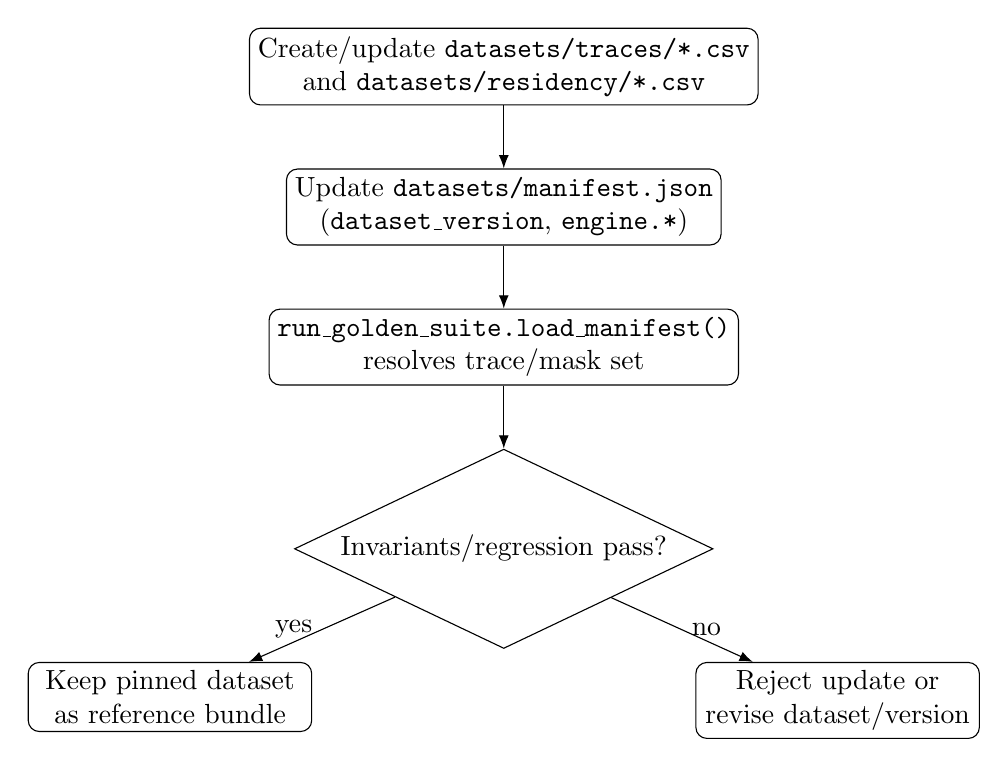
\begin{tikzpicture}[node distance=8mm and 11mm]
\node[box] (a) {Create/update \texttt{datasets/traces/*.csv}\\and \texttt{datasets/residency/*.csv}};
\node[box, below=of a] (b) {Update \texttt{datasets/manifest.json}\\(\texttt{dataset\_version}, \texttt{engine.*})};
\node[box, below=of b] (c) {\texttt{run\_golden\_suite.load\_manifest()}\\resolves trace/mask set};
\node[decision, below=of c] (d) {Invariants/regression pass?};
\node[box, below left=of d] (e1) {Keep pinned dataset\\as reference bundle};
\node[box, below right=of d] (e2) {Reject update or\\revise dataset/version};
\draw[line] (a) -- (b);
\draw[line] (b) -- (c);
\draw[line] (c) -- (d);
\draw[line] (d) -- node[left]{yes} (e1);
\draw[line] (d) -- node[right]{no} (e2);
\end{tikzpicture}
\caption{Reference Datasets Function Flow}
\end{figure}

\end{document}
